%% LyX 2.2.0 created this file.  For more info, see http://www.lyx.org/.
%% Do not edit unless you really know what you are doing.
\documentclass[english,aps,pre, reprint, twocolumn]{revtex4}
\usepackage[T1]{fontenc}
\usepackage[latin9]{inputenc}
\setcounter{secnumdepth}{3}
\usepackage{graphicx}

\makeatletter
%%%%%%%%%%%%%%%%%%%%%%%%%%%%%% Textclass specific LaTeX commands.
\@ifundefined{textcolor}{}
{%
 \definecolor{BLACK}{gray}{0}
 \definecolor{WHITE}{gray}{1}
 \definecolor{RED}{rgb}{1,0,0}
 \definecolor{GREEN}{rgb}{0,1,0}
 \definecolor{BLUE}{rgb}{0,0,1}
 \definecolor{CYAN}{cmyk}{1,0,0,0}
 \definecolor{MAGENTA}{cmyk}{0,1,0,0}
 \definecolor{YELLOW}{cmyk}{0,0,1,0}
}

\makeatother

\usepackage{babel}
\begin{document}

\preprint{\%This line only printed with preprint option}

\title{Assembly and manipulation of mesoscopic particles by active thermocapillary
stress}

\author{Basudev Roy}

\affiliation{Indian Institute of Science Education and Research, Kolkata }

\author{Rajesh Singh}

\affiliation{Institute of Mathematical Sciences, Chennai}

\author{Subhrokoli Ghosh}

\affiliation{Indian Institute of Science Education and Research, Kolkata }

\author{Ronojoy Adhikari}
\email{ronojoy.adhikari@gmail.com}


\affiliation{Institute of Mathematical Sciences, Chennai}

\author{Ayan Banerjee}
\email{ayan@iiserkol.ac.in}


\affiliation{Indian Institute of Science Education and Research, Kolkata }
\begin{abstract}
The temperature variation of the surface tension at a liquid-gas interface
generates tangential thermocapillary stresses which produce flows
in the ambient fluid. Here, we demonstrate that such active stresses
can be produced in a controlled manner by inducing a microbubble in
optical tweezers. An analytical solution of the thermocapillary problem,
based on the Stokes and heat equations, yields the flow profile around
the bubble. It is clear that under the action of the resulting flow,
mesoscopic particles dispersed in the ambient fluid assemble in in
rings at the bubble interface. We proceed to demonstrate this experimentally
by inducing self-assembly of polystyrene microparticles on the bubble
surface in rings. In addition, we show transport of a wide range of
particles ranging from gold nanoparticles to polystyrene microspheres
using thermophoretic motion of the bubble under translation of the
optical tweezers. Most importantly, we are able to release particles
captured on the bubble surface by modulating the bubble diameter controllably.
We also study the flow fields around a pair of microbubbles theoretically
and observe that these would allow for additional control on particle
assembly and manipulation. We realize the theoretical predictions
experimetally by growing two microbubbles adjacent to each other and
modifying the trajectory of freely diffusing polystyrene microparticles
which are in the vicinity of the bubbles. Our studies indicate that
the active thermocapillary stresses induced by multiple microbubbles
could offer routes to particle micromanipulation that would otherwise
be difficult to achieve in optical tweezers. 
\end{abstract}
\maketitle

\section{introduction}

The study of active stress on mesoscopic particles in fluidic environments
has evoked widespread scientific interest in recent times since it
enables the understanding and ultimate control of fundamental processes
involving fluid-particle interactions at a microscopic level, and
leads to a variety of applications. The fundamental processes range
from transport of organelles inside the fluidic environment in a cell
{[}1{]}, to the motion of cilia and flagella of swimming bacteria
{[}2{]}. The analysis of the active stress involved in many such processes
has led to the design of ``active'' particles {[}3{]}, that often
mimic natural microswimmers. These active particles move in pre-designed
paths by interacting with their environment and exchanging energy
by diverse processes including thermophoresis {[}4{]}, electrophoresis
{[}5{]}, diffusiophoresis {[}6{]}, etc. Such controlled motion of
mesoscopic particles under different active stress has very significant
implications in different areas including cell biology {[}7{]}, nanomedicine
{[}8{]}, and micro-patterning {[}9{]}. Active stress can also be induced
on microparticles in a fluid by manipulating the flow environment
using different techniques of actuation {[}10{]} in microfluidic channels,
and by generating surface stresses by controlled modulation of fluid-fluid
or fluid-solid boundaries. The latter can be achieved by a number
of processes such as electrowetting {[}11{]}, thermocapillary action
{[}12{]}, and Marangoni stresses {[}13{]}.

Recently, it has been show that the thermocapillary flow around a
thermooptically generated bubble can be used to trap silica particles
and nanotubes. These bubbles are generated by focusing the trapping
laser on an absorbing substrate on the wall of a water filled trapping
chamber. The rapid heating causes the water in the vicinity of the
laser ``hot spot'' to spinodally decompose and grow into a bubble.
The bubble reaches a steady state size determined by the laser power
and remains thermophoretically trapped in the region of the temperature
maximum. Since there is an appreciable temperature difference between
the pole of the bubble which is in direct contact with the hot spot
and its opposite pole which is farthest from the hot spot, an active
Marangoni stress is immediately developed on the bubble surface. This
active stress drives fluid flow towards the bubble and away from the
wall. Particles are drawn towards the bubble due to this convective
flow and attach to the bubble surface {[}14,15,18{]}. The hot spot
can be translated and the bubble, driven by the strong thermophoretic
forces, follows it. This provides a method for transporting particles
that are attached to the bubble surface. 

Such thermophoretic trapping mechanisms have several advantages of
over standard optical tweezers. First, thermophoretic traps are agnostic
to the dielectric constrast between the particle and the suspending
medium. Thus, particles with negative dielectric constrast that are
impossible to trap using standard optical means can easily be trapped
thermophoretically. Second, thermophoretic traps can apply nN forces
while optical traps can only apply much weaker forces in the range
of a few hundred pN. Third, thermophoretic traps can transport multiple
particles over large distances stably and simultaneously. While such
trapping and manipulation by attaching particles to the bubble surface
has been experimentally demonstrated, a controllable and consistent
method for detaching the particles from the bubble surface without
destroying the bubble is yet to be shown. This renders this otherwise
robust particle transportation technique somewhat incomplete. Further,
a clear picture of the active stress driven hydrodynamic flow is lacking.
In this paper, we address both these issues. By solving the Navier
Stokes and heat equations, we calculate the exact flow pattern of
liquid around a laser induced microbubble. We go on to show how the
flow pattern may be modified by having two bubbles adjacent to each
other, and the implications on particle motion. Experimentally, we
demonstrate interesting and reproducible self assembly of polystyrene
beads of different sizes on the bubble surface - a phenomenon that
is easily explained by our theoretical simulations. We also develop
a technique for controllable release and attachment of particles to
a bubble by modulating the bubble size, and proceed to demonstrate
capture, transport, and release of gold and silver nanoparticles using
a single microbubble. Finally, we provide a glimpse of the fascinating
possibilities of manipulating the trajectories of micro-particles
by trapping two micro-bubbles adjacent to each other, and observing
particle trajectories in their vicinity. We believe that with proper
choice of micro-bubble sizes and separations, this method can be eventually
used as a tunable particle sorter - having the capability of sorting
particles of different sizes continuously, since the bubble sizes
and separations can be continuously tuned.

\section{Theory}

We describe the system with a set of equations assuming a steady state,
which are: 

1. The Navier-Stokes equation describes the velocity of the fluid
flow in the system: 

\begin{equation}
\nabla P+\eta\nabla^{2}\mathrm{\mathit{v}=}0
\end{equation}

2. Incompressibility condition:

\begin{equation}
\nabla.v=0
\end{equation}

3. Heat equation:

\begin{equation}
\nabla^{2}\mathrm{\mathit{T}=}0
\end{equation}

Here $\mathit{v,}$ $\mathit{P,}$ and $\mathit{T}$ are the fluid
velocity, pressure and temperature respectively. These set of equations
have to solved together with a set of boundary conditions. These are:
\begin{enumerate}
\item $v=0$ on the wall.
\item T = Room temperature at wall.
\item $v\rightarrow0$ at $x=\infty$.
\item $p\rightarrow$constant at $x=\infty$.
\item $\nabla T$ is along $\mathit{z}$ at $x=\infty$. 
\end{enumerate}
There are another set of boundary conditions on the bubble wall that
balances stresses: 
\begin{enumerate}
\item $v.n=0$ on the surface of the bubble (no flow into the bubble).
\item $n.\nabla T=0$ on the bubble surface (temperature gradient is only
tangential).
\item Tangential stress = Normal temperature gradient (Marangoni condition). 
\end{enumerate}

\section{experimental results\label{sec:expres}}

The thermo-optic tweezers setup is based on an inverted Zeiss Axiovert.A1
microscope with a 100x 1.41 NA lens objective lens focusing the tweezers
laser beam at 1064 nm into the sample chamber containing an aqueous
dispersion of the sample (usually polystyrene microspheres of different
diameters). We use two types of absorptive surfaces in the sample
chamber: 1. A surface that is pre-coated by linear trails of a Mb-based
soft oxometalate (SOM) material by a method developed by us (see Ref.
{[}19{]}). The SOM material has finite absorption at 1064 nm, so that
a hot spot is formed leading to a bubble when the tweezers laser is
focused on any region along the trail. 2. A gold coated surface. We
typically make abrasions on the gold coating with a sharp knife edge
in order to create irregularities on the surface that can act as nucleation
centers for bubble growth. The laser creates a hot spot due to enhanced
absorption resulting from local plasmonic excitation, as a result
of which the water gets heated above the boiling point to create a
bubble. The absorptive surface (typically a microscope slide which
forms the top surface of the chamber) is attached to a cover slip
(bottom surface) by sticky tape. In both cases, the temperature of
the hot spot would vary between around 373K (the threshold for bubble
formation) to 644K - the latter corresponding to the critical temperature
for water after which it cannot exist as a liquid with the surface
tension tending to zero. The temperature of the hot spot can be modified
by changing the laser intensity incident on it, which we typically
achieve by changing the laser power. 

\subsection{Self assembly of particles on bubbles:\label{subsec:selfassem}}

Once the bubble is formed, convective flows set in which draw particles
towards it. As shown in the simulation results in Fig. 1, the flow
lines tend to converge along an equatorial circle of the bubble, so
that we have an assembly of particles near that region. This is shown
in Fig. 2, where we have a bubble of around 10 $\mu\mathrm{m}$in
diameter formed along a SOM trail in a sample chamber of the first
type. 3 $\mu\mathrm{m}$ diameter polystyrene beads in aqueous dispersion
follow the flow lines and assemble with time as shown in Fig. 2a -
d. Video 1 in the multimedia files of the Supplementary Information
shows the entire process in real time. We observe self assembly of
a variety of particles including polystyrene beads of diameter 1,
3, and 10 $\mu\mathrm{m}$ (Video 2), as well as other particles including
streptavidin coated magnetic beads of diameter 3 $\mu\mathrm{m}$
(Video 3), and gold (Video 4) and silver nanoparticles (Video 5) of
around 10-100 nm in size. Note that the latter are notoriously difficult
to trap using conventional optical tweezers due to their large scattering
cross-sections. However, using this technique the scattering is rendered
irrelevant since the particles are not exposed to light at all.

\begin{figure}[h]
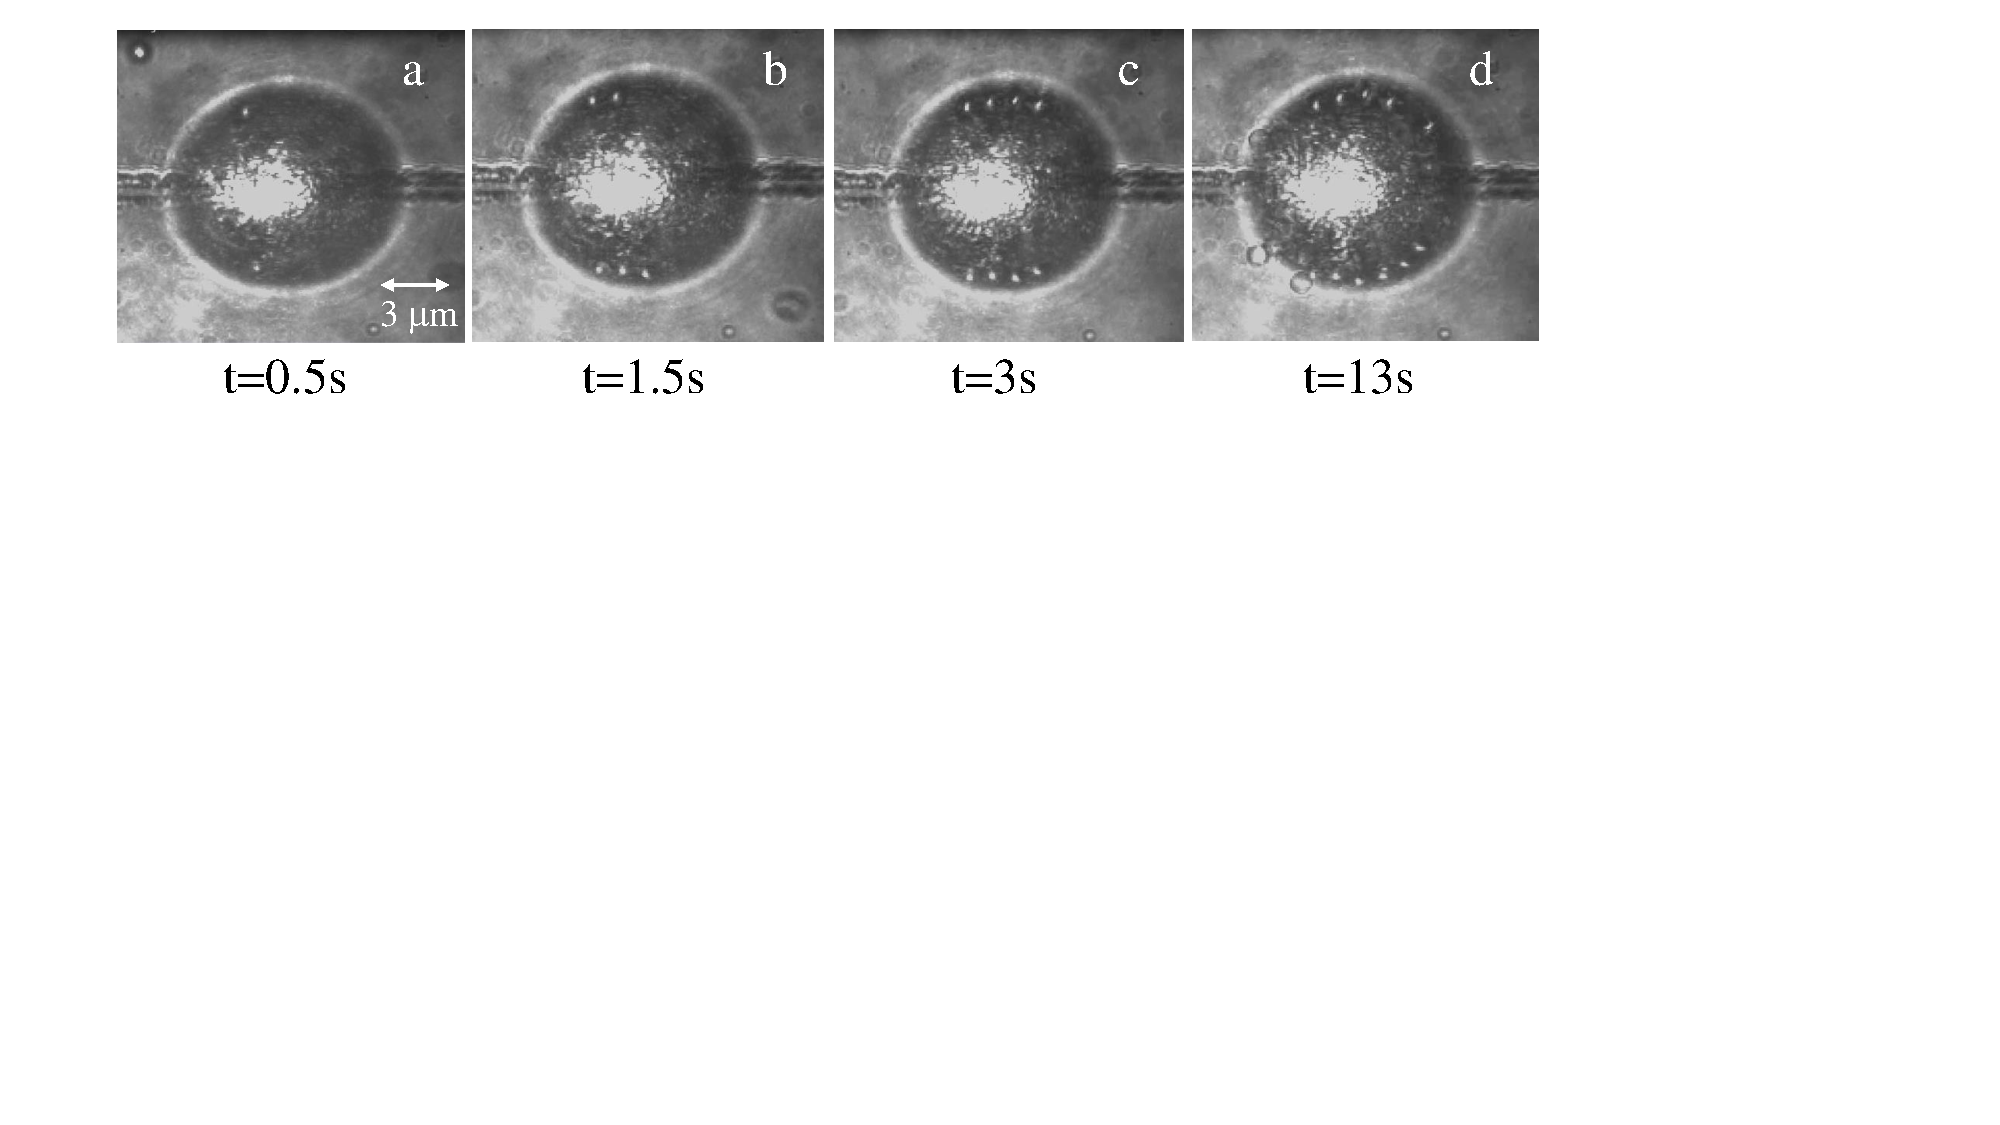
\includegraphics[draft,clip,scale=0.4]{figures/Figure2}

Figure 2. Time lapse images of 3 $\mu\mathrm{m}$ diameter polystyrene
beads in aqueous dispersion assembling on a bubble of diameter around
10 $\mu\mathrm{m}$ grown on a SOM trail. The beads follow flow lines
and assemble along an equatorial circle around the bubble. We see
around 2 beads in panel a which is at t=0.5 s, while around 14 beads
are distinctly visible in d, which is at t=13 s. These have been extracted
from Video 1 in the multimedia files of the Supplementary Information.
\end{figure}


\subsection{Translation of bubbles with particles loaded\label{bubbletrans}}

We are able to transport the particles thus assembled on the bubble
as is shown in Videos 2-5 in the Supplementary Information. These
include polystyrene beads, magnetic beads and nanoparticles as described
in the earlier sections. The bubble is moved by translating the laser
along the absorptive surface (of both types as described in Sec.\ref{sec:expres})
on which the bubble is initially formed. The translation of the laser
translates the hot spot as a result of which the Marangoni flows push
the bubble in the direction of the higher temperature. We are able
to translate bubbles with particles loaded on their surface with velocities
of the order of 5 mm/s. Note that the translation of the polystyrene
beads were performed on a SOM trail, while the gold and silver nanoparticles
were moved along a gold surface.

\subsection{Particle capture and release \label{partcapt}}

Translation of bubbles with particles loaded on the surface has been
demonstrated recently in Refs. {[}14,15{]}. Generally, particle release
is performed by switching off the laser so that the bubble gradually
collapses. However, we demonstrate a method of particle release without
destroying the bubble, as is shown in Fig. 3. Here, we actually modulate
the laser intensity by applying a square pulse to the laser current
driver so that the power output of the laser changes according to
the pulse amplitude. This causes the bubble diameter to change in
sync with the laser power. Now, when the bubble diameter reduces so
as to increase the radius of curvature of the bubble, the concomitant
increase in surface energy is reduced by expelling the particles in
contact with the bubble. Thus, the additional surface area due to
the particles attached to the bubble is also reduced so that the energy
is indeed minimized. Figure 3 shows time lapsed images of 3 $\mu\mathrm{m}$
diameter polystyrene beads being released and recaptured by the bubble
due to the modulation of the bubble size. As the bubble diameter is
reduced to a certain critical size, the particles are released, only
to be recaptured once the bubble is back to the initial size. It is
expected that larger particles would require a smaller bubble size
to be released since they have larger surface area with a higher sticking
force on the bubble surface. 

\begin{figure}[t]
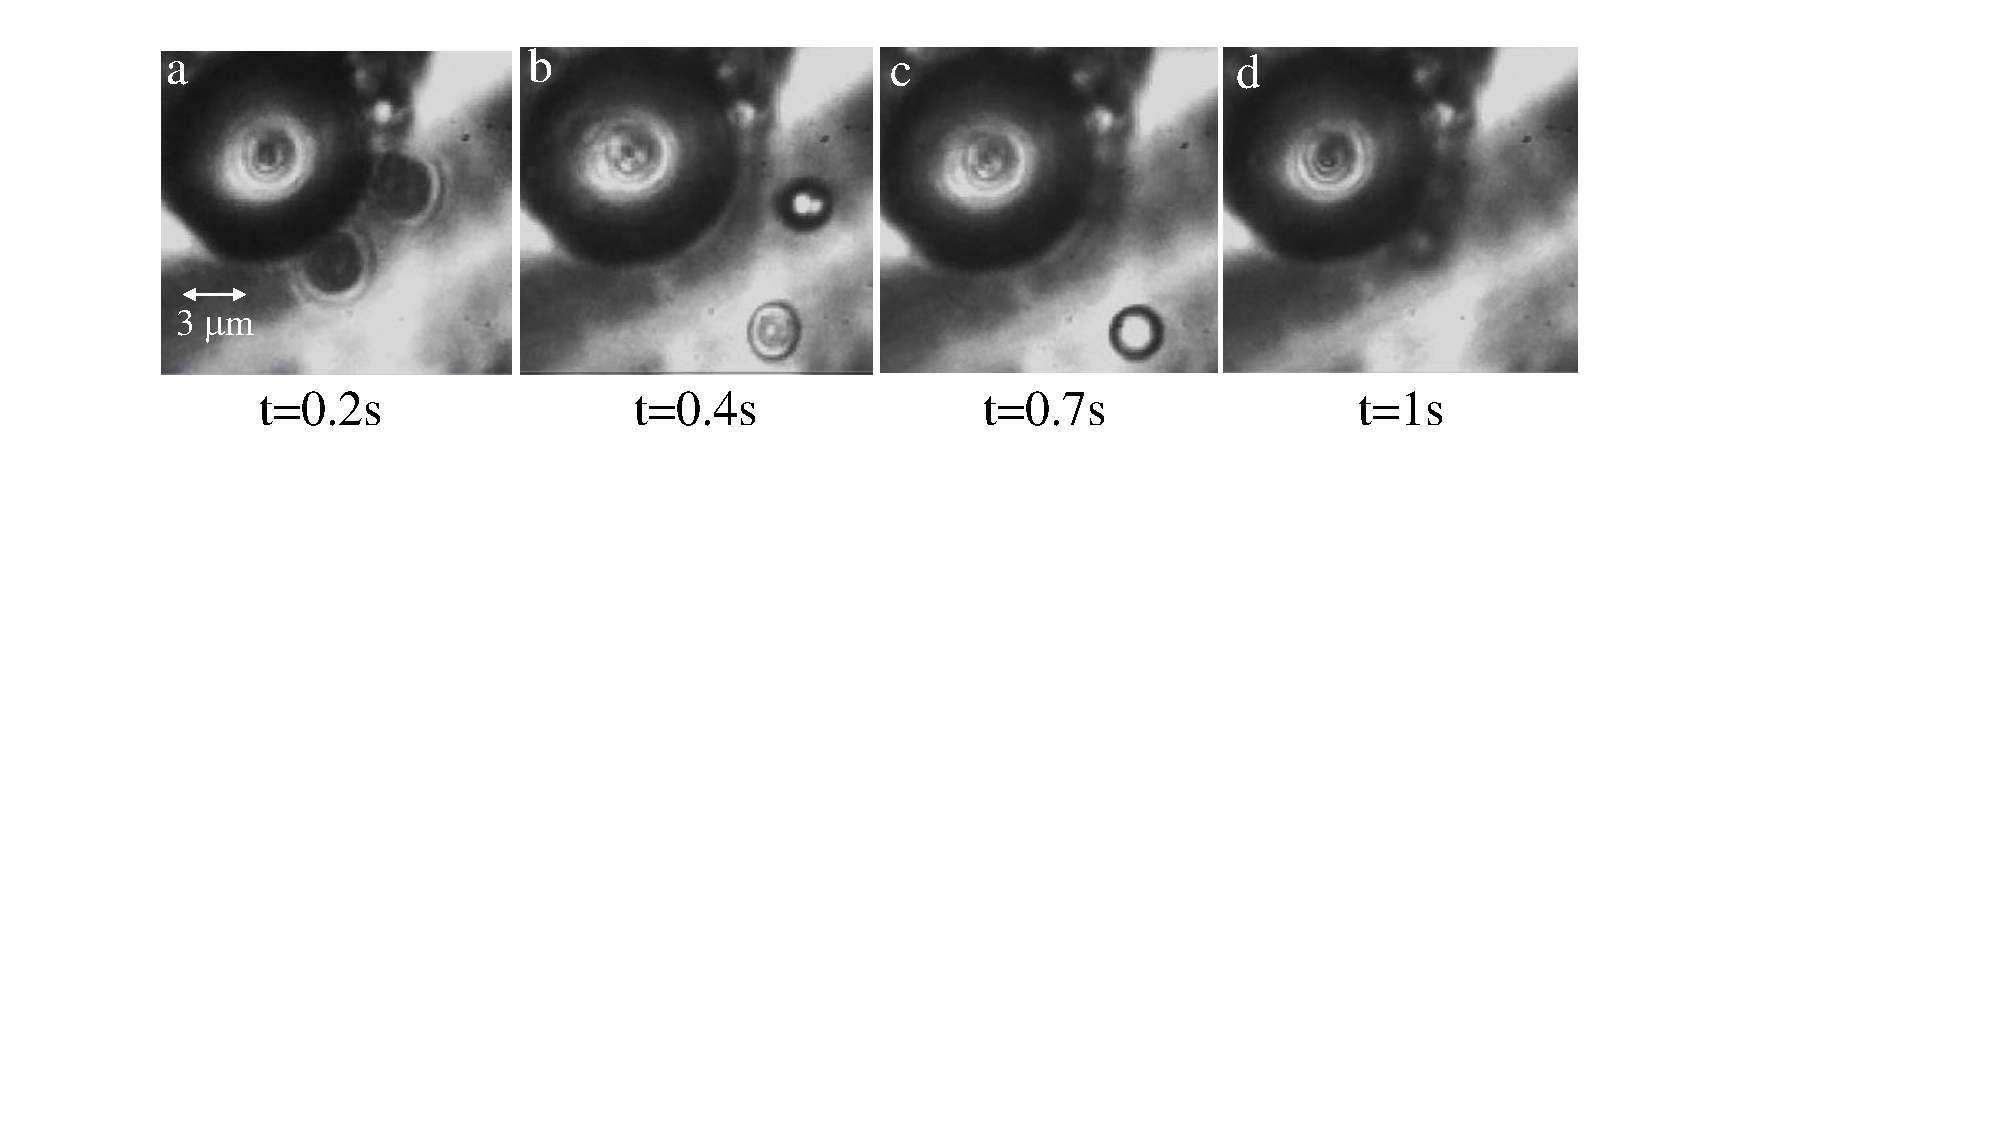
\includegraphics[scale=0.4]{figures/Figure3}

Figure 3. Time lapsed images of particle release and recapture by
modulation of the bubble size. The particles are 3 $\mu\mathrm{m}$
diameter polystyrene beads. a) Two beads attached to the surface.
b) Both have been released by changing the bubble size (see Video
6 in Supplementary Information). The bead at the bottom right corner
is at a different z-depth compared to the bead closer to the bubble,
so that they appear to be of different sizes since the focusing is
different. c) The bead nearer to the bubble is back to the bubble
surface (seen as a blur due at the side of the bubble due to different
z-depth again), while the one farther away is still free. 4) The bead
farther has been recaptured by the bubble (seen as a blur at the side
once more). 
\end{figure}


\subsection{Particle manipulation using two bubbles \label{partmanipulate}}

In these set of experiments, we created two adjacent bubbles on neighbouring
pre-existing SOM trails. The bubbles are shown in Fig. 4, of size
around 24 and 28 $\mu\mathrm{m}$ respectively. The flow pattern around
the bubbles are demonstrated in the simulation shown in Fig. 1b. To
verify this flow pattern we have particles of diameter 3 $\mu\mathrm{m}$
in the aqueous dispersion, and their trajectories are highlighted
in Fig. 4. It is clear that a separatrix can be identified between
the two bubbles, and particles would be drawn towards a bubble depending
on whether its trajectory lies above or below the separatrix. The
position of the separatrix is modified with the change in size of
the bubbles, as is apparent from simulations as shown in Fig. 1b.
We can thus envisage the use of this technique to generally sort particles
by size modulation of the two bubbles, where the position of the separatrix
would be continuously modulated by changing the laser power, so that
by a suitable choice of separation between the bubbles and modulation
frequency, one can allow particles of a certain diameter to pass between
the bubbles while others would be trapped on the bubble surfaces.
We are currently working on some of these experiments.

\section{Conclusions}
\begin{acknowledgments}
Thank you so much!
\end{acknowledgments}

\begin{thebibliography}{1}
\bibitem{mycitation}Author, ``Title'', Journal \textbf{Volume},
page\textendash numbers (year).
\end{thebibliography}

\end{document}
